\documentclass[Report.tex]{subfiles}

\begin{document}

\chapter{Theory}
This chapter gives an overview on the theoretical background of the
methods used during image processing, clustering the lines and pattern matching.
\label{chapter:Theory}

\section{Image Processing} % (fold)
\label{sec:Image Processing}
The image processing contains the following steps:
\begin{itemize}
  \item converting the image captured from the camera into grayscale,
  \item applying threshold function,
  \item finding edges in the filtered image using the Canny edge detection,
  \item transforming the edges to a bird's eye view image,
  \item finding line segments in the bird's eye view image by a
    probabilistic Hough transform algorithm.
\end{itemize}
All these steps except the bird's eye view transformation were performed by some certain
OpenCV\cite{www:opencv} function calls. Figure \ref{fig:img_proc} shows the input and output
images for each step. The Hough transformation image shows the Hough lines with
red color and the end points of each line with blue.

\begin{figure}[hp]
  \centering
  \setlength\fboxsep{2pt}
  \setlength\fboxrule{0pt}

  \fbox{
    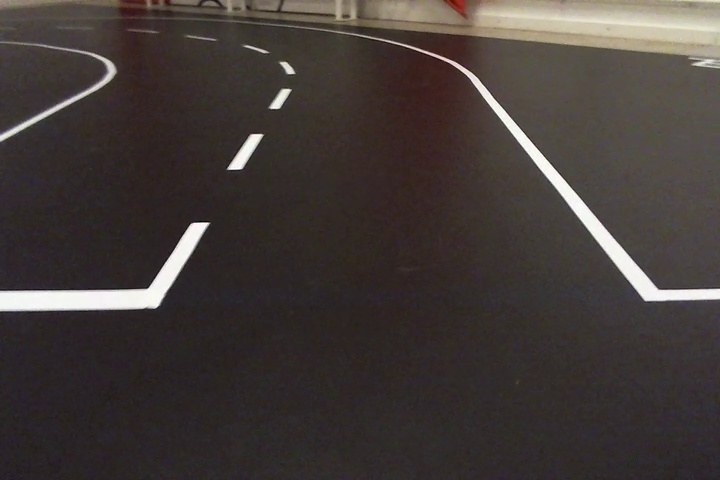
\includegraphics[width=0.5\textwidth]{figures/1_original.jpeg}
    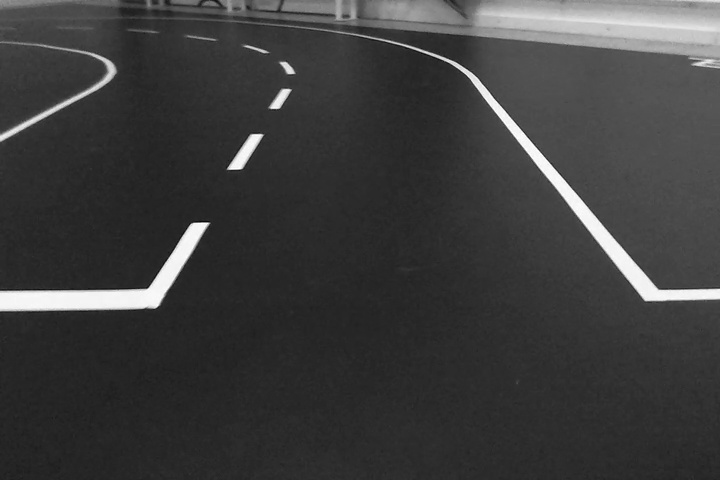
\includegraphics[width=0.5\textwidth]{figures/2_grayscale.jpeg}
  }
  \fbox{
    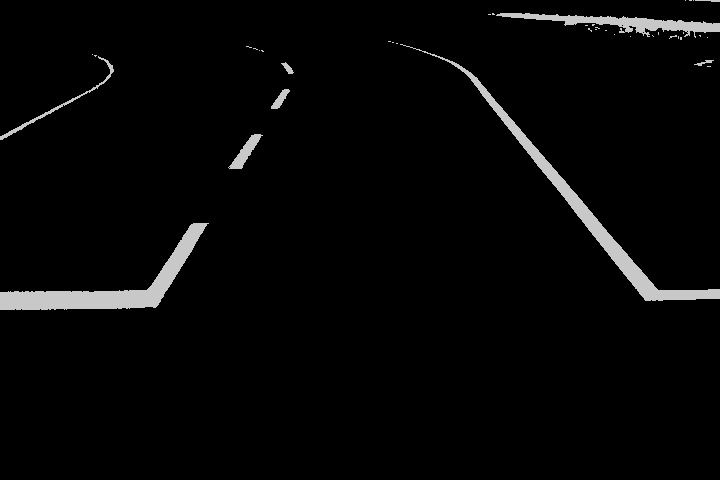
\includegraphics[width=0.5\textwidth]{figures/3_threshold.jpeg}
    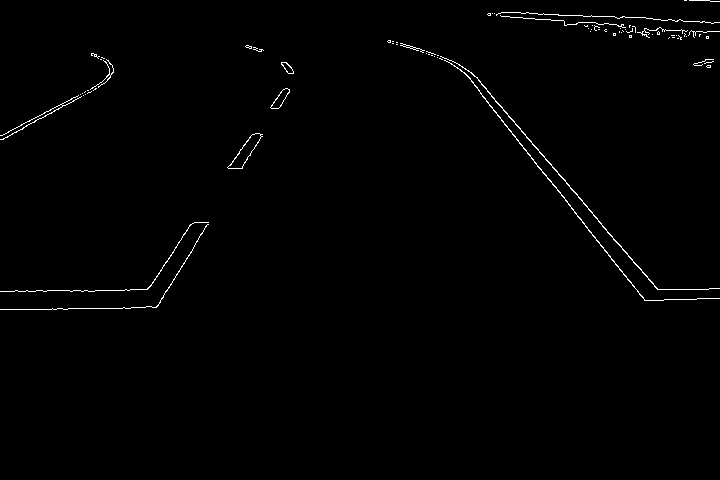
\includegraphics[width=0.5\textwidth]{figures/4_canny.jpeg}
  }
  \fbox{
    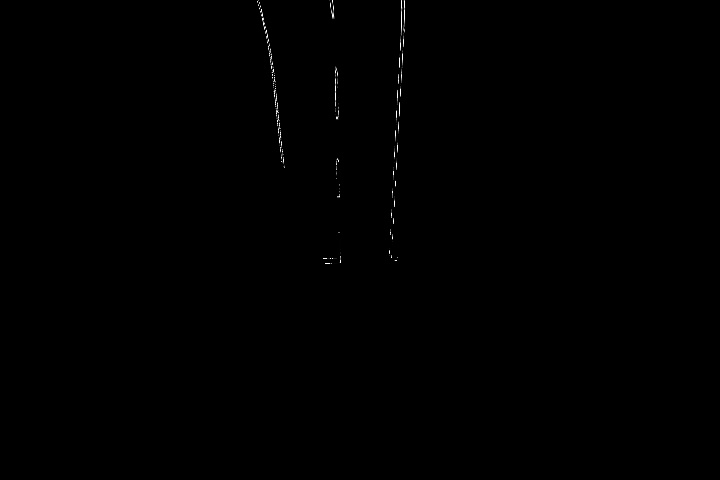
\includegraphics[width=0.5\textwidth]{figures/5_birdview.jpeg}
    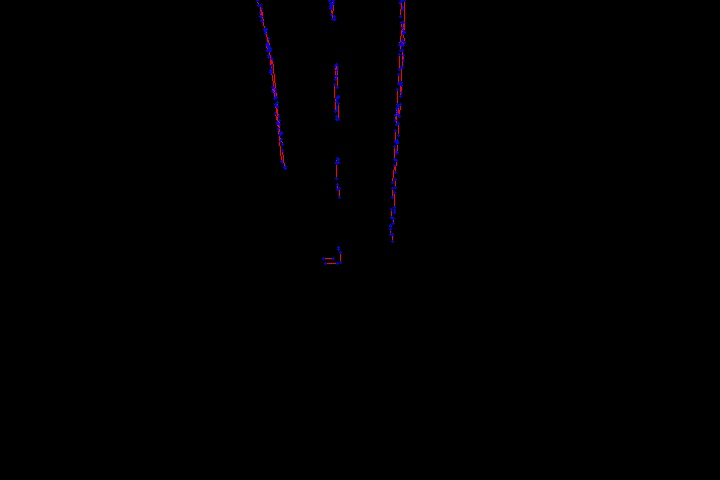
\includegraphics[width=0.5\textwidth]{figures/6_hough.jpeg}
  }
  \caption{Stages of image processing (top-left: original, top-right:
  grayscale, middle-left: threshold, middle-right: canny edge-detection,
bottom-left: bird's eye view, bottom-right: Hough transform)}
  \label{fig:img_proc}
\end{figure}

As for the bird's eye view transformation\cite{article:bird}, it has two
separate phases. The first phase is to generate the transformation matrix M,
while the second phase is to fed this matrix M to the
warpPerspective\cite{www:warp} OpenCV function.  The following equations show
the calculation of this matrix M:

\normalsize
\[
A1=
\begin{bmatrix}
  1 & 0 & -\frac{img.width}{2} & \\
  0 & 1 & -\frac{img.height}{2} & \\
  0 & 0 & 0 & \\
  0 & 0 & 1 &
\end{bmatrix}
A2=
\begin{bmatrix}
  f & 0 & \frac{img.width}{2} & \\
  0 & f & \frac{img.height}{2} & \\
  0 & 0 & 0 & \\
  0 & 0 & 1 &
\end{bmatrix}
T=
\begin{bmatrix}
  1 & 0 & 0 & 0 & \\
  0 & 1 & 0 & 0 & \\
  0 & 0 & 1 & distance & \\
  0 & 0 & 0 & 1 &
\end{bmatrix}
\]
\[
R_{x}=
\begin{bmatrix}
  1 & 0 & 0 & 0 & \\
  0 & cos(\alpha) & -sin(\alpha) & 0 &  \\
  0 & sin(\alpha) & cos(\alpha) & 0 &  \\
  0 & 0 & 0 & 1 &
\end{bmatrix}
R_{y}=
\begin{bmatrix}
  0 & cos(\beta) & -sin(\beta) & 0 &  \\
  0 & 1 & 0 & 0 & \\
  0 & sin(\beta) & cos(\beta) & 0 &  \\
  0 & 0 & 0 & 1 &
\end{bmatrix}
R_{z}=
\begin{bmatrix}
  cos(\gamma) & -sin(\gamma) & 0 & 0 & \\
  sin(\gamma) & cos(\gamma) & 0 & 0 & \\
  0 & 0 & 1 & 0 & \\
  0 & 0 & 0 & 1 &
\end{bmatrix}
\]

\[
R=R_{x}*R_{y}*R_{z}
\]

\[
M = A2*(T*(R*A1))
\]
\Large

First of all, the matrix \textit{A1} shifts the image in the coordinate system such that its center is located at (0,0).
Secondly, the rotational matrix \textit{R} can be calculated from \textit{$R_{x}, R_{y}$}
and \textit{$R_{z}$} matrices.  Thirdly, the translation matrix \textit{T} can adjust
the height of the camera position by the \textit{distance} parameter. Lastly, the
warpPerspective OpenCV function is called with the WARP\_INVERSE\_MAP parameter
which calculates the final image as follows:
\normalsize
\[BirdView(x,y)= warpPerspective(inputImg, M, WARP\_INVERSE\_MAP) = \]
\[= inputImg*(\frac{M_{11}x+M_{12}y+M_{13}}{M_{31}x+M_{32}y+M_{33}},\frac{M_{21}x+M_{22}y+M_{23}}{M_{31}x+M_{32}y+M_{33}})\]
\Large
% section Image Processing (end)

\section{Line Clustering} % (fold)
\label{sec:Line Clustering}
For clustering lines a modified DBSCAN\cite{www:dbscan} algorithm was used. Originally
DBSCAN operates on a set of points and returns a set of clusters of points.
Since in our case the input data is a set of lines, this algorithm must be
adapted to this type of input data. It is done by checking if any end point of
a line is density-connected to any point of a cluster, and if so, then it adds both end
points to that cluster, not just the one that is actually connected to the
cluster.  Two points are density-connected if there is a third point such that
those two points are reachable from that third point and each of these points
has a sufficient amount of neighbours to form a cluster.
A cluster satisfies two properties:
\begin{itemize}
  \item all points within the cluster are mutually density-connected,
  \item if a point is density-connected to any point of the cluster, it is part
of the cluster as well.
\end{itemize}
There are two parameters for this algorithm. The minimum number of lines
required to form a cluster, and epsilon which defines the minimum distance
between clusters.
Code~\ref{pseudo:dbscan} shows the pseudo code for the DBSCAN clustering
algorithm used in this project.

\begin{code}[hp]
\large
\begin{verbatim}
DBSCAN(D, eps, MinLines)
   C = 0
   for each unvisited line L in dataset D
      mark L as visited
      NeighborLines = regionQuery(L, eps)
      if sizeof(NeighborLines) < MinLines
         mark L as NOISE
      else
         C = next cluster
         expandCluster(L, NeighborLines, C, eps, MinLines)

expandCluster(L, NeighborLines, C, eps, MinLines)
   add L to cluster C
   for each point L' in NeighborLines
      if L' is not visited
         mark L' as visited
         NeighborLines' = regionQuery(L', eps)
         if sizeof(NeighborLines') >= MinLines
            NeighborLines = NeighborLines joined with NeighborLines'
      if L' is not yet member of any cluster
         add L' to cluster C

regionQuery(L, eps)
   return all lines within L's eps-neighborhood (including L)
\end{verbatim}

\caption{DBSCAN clustering algorithm}
\label{pseudo:dbscan}
\end{code}
% section Line Clustering (end)

\section{Pattern Matching} % (fold)
\label{sec:Pattern Matching on Clusers}
Pattern matching is needed to identify the clusters that cover the dashed line
and the two solid lines on the lane. The current implementation uses a very
basic approach. That is checking the maximum difference on the x and y axes
between each pair of nodes and comparing these maximum values to a predefined
threshold value. The maximum x value must be lower than the threshold for x,
while the maximum y value must be higher than the threshold of y. In case of
dashed lines, the maximum x value must fall into a range of acceptable values,
since the length of dashes is fix and known. The only aim of this basic check
is to find the line shaped clusters.
% section Pattern Matching on Clusers (end)

\end{document}
